\documentclass[twoside]{report}
\usepackage{graphicx}
\usepackage{fancyhdr}
\usepackage{xcolor}

\begin{document}
\raggedright{}
Dieser \textit{schöne} Beispieltext \textbf{zeigt} verschiedene \underline{Schriftschnitte}.\\
\textit{Dieser ganze Text ist kursiv, soll aber trotzdem noch ein \emph{Wort} hervorheben.}\\

\vspace{1cm}

\centering{Dieser Satz ist zentriert.}\\

\raggedright{Der Satz ist linksbündig.}\\

\raggedleft{Der Satz ist rechtsbündig.}\\
%neuer Absatz durch \\ oder \newline.
\raggedright{}

\vspace{1cm}

\pagestyle{fancy}
\fancyhead[RO,LE]{Diese Kopfzeile wird auf ungeraden Seiten rechts und auf geraden links angezeigt.}
%Kapitel und Kopfzeilen sind nur in der Dokumentenklasse book vereinbar.
\fancyfoot[RO,LE]{Weder Kopfzeilen noch Fußnoten sind mit Kapiteln verträglich.}
\cfoot{}

\large{Der ganze Satz ist größer als der nächste.}\\

\small{Der Satz ist kleiner als der erste.}

\vspace{1cm}

\begin{figure}[h]
    \centering
    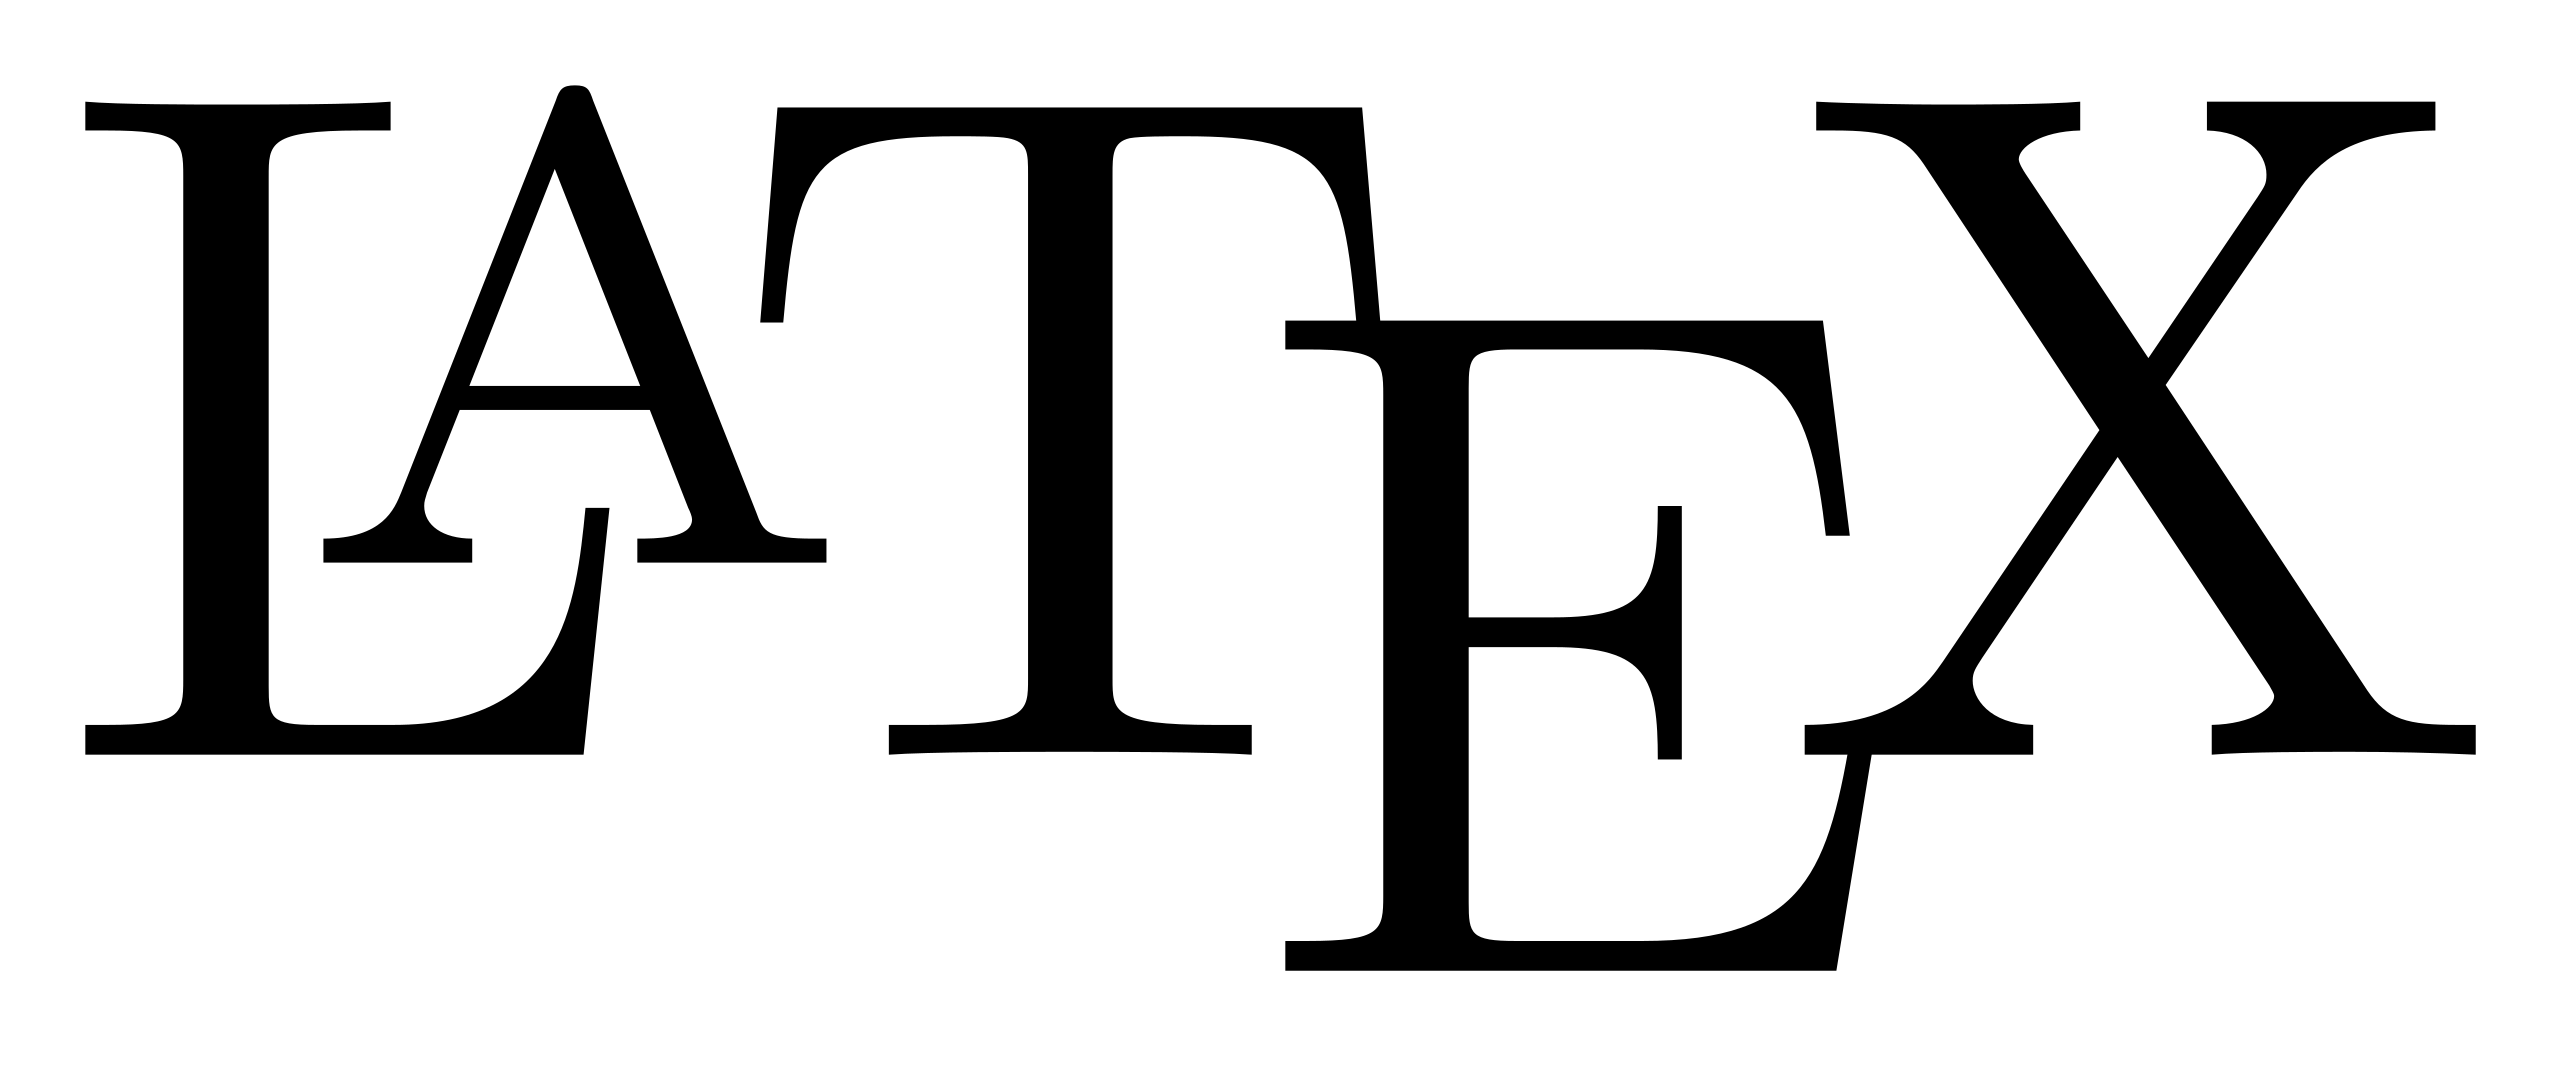
\includegraphics[width=\textwidth]{Bild1/LaTeX1.png}
    \caption{Das ist das \LaTeX{}-logo.}
    \label{fig:LaTeX1.png}
\end{figure}
Nun möchte ich auf das \LaTeX{}-logo hinweisen, welches sie in Graphin \ref{fig:LaTeX1.png} sehen.\\


\vspace{1cm}
%Abstände

So werden andere Dateien eingefügt.

\vspace{1cm}


Nun habe ich euch bereits etwas über:
\begin{itemize}
    \item Schriftschnitte
    \item Schriftgrößen
\end{itemize}

\begin{enumerate}
    \item Graphiken
\end{enumerate}
erzählt.

\vspace{4cm}

Formel für den Flächeninhalt eines Kreises:
\[A=\pi×r^2\]

\vspace{1cm}


Tabellen:\\
\vspace{0.5cm}
\begin{tabular}{||c|c|c||}
\hline\hline
cell1 & cell2 & cell3\\
\hline
cell4 & cell5 & cell6\\
\hline
cell7 & cell8 & cell9\\
\hline\hline
\end{tabular}

\chapter{Erstes Kapitel}
\section{Erster Abschnitt}
\subsection{Erster Unterabschnitt}

\color{blue}

\chapter*{Erstes Kapitel}
\section*{Erster Abschnitt}
\subsection*{Erster Unterabschnitt}



\end{document}
